\documentclass[border=4pt]{standalone}
\usepackage{amsmath,amssymb,amsfonts}
\usepackage{xcolor,colortbl,array,booktabs,multirow}
\usepackage{tikz}
\usetikzlibrary{arrows, automata, backgrounds, calendar, chains, decorations,
    matrix, mindmap, patterns, petri, positioning, shadows, shapes.geometric,
    trees, shapes, decorations.pathreplacing, calc, tikzmark, arrows.meta}
\newcommand{\st}{\text{ s.t. }}
\newcommand{\x}{\mathbf{x}}
\renewcommand{\b}{\mathbf{b}}
\newcommand{\A}{\mathbf{A}}
\newcommand{\R}{\mathbb{R}}
\newcommand{\RR}{\mathbb{R}}
\newcommand{\Z}{\mathbb{Z}}
\newcommand{\ZZ}{\mathbb{Z}}
\begin{document}
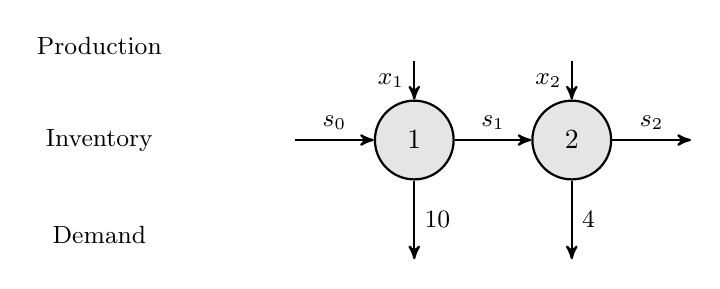
\begin{tikzpicture}[
    node distance=2cm, 
    thick, 
    >=stealth',
    every node/.style={font=\small},
    main/.style={circle, draw, fill=gray!20, minimum size=1cm, font=\normalsize}
]

% Nodes
\node[main] (1) {1};
\node[main, right of=1] (2) {2};

% Arrows for Production
\draw[->] (1) ++(0,1) -- node[left] {$x_1$} (1.north);
\draw[->] (2) ++(0,1) -- node[left] {$x_2$} (2.north);

% Arrows for Inventory
\draw[<-] (1.west) -- ++(-1,0) node[midway, above] {$s_0$};
\draw[->] (1.east) -- node[midway, above] {$s_1$} (2.west);
\draw[->] (2.east) -- ++(1,0) node[midway, above] {$s_2$};

% Arrows for Demand
\draw[->] (1.south) -- ++(0,-1) node[midway, right] {10};
\draw[->] (2.south) -- ++(0,-1) node[midway, right] {4};

% Labels
\node at (-4,1.2) {Production};
\node at (-4,0) {Inventory};
\node at (-4,-1.2) {Demand};

\end{tikzpicture}
\end{document}
